\documentclass{article}
\usepackage[utf8]{inputenc}
\usepackage[margin=0.8in]{geometry}

%\biboptions{sort&compress} %Change citations to be 1-10 if lots are listed

\usepackage{amsmath}
\usepackage{amsfonts} 
\usepackage{amssymb}
\usepackage{bm}
\usepackage{hyperref}

%For tables
\usepackage{booktabs}
\usepackage{multirow}
\usepackage{graphicx}

%For images
\graphicspath{{images/}}

%For subfigures
\usepackage{caption}
\usepackage{subcaption}

%For different coloured text
\usepackage{xcolor}

%For the bibliography
\usepackage[backend=biber,
style=ieee,
sortcites=true,
sorting=none]{biblatex}

%citestyle=numeric-comp,
%bibstyle=authoryear,       
\addbibresource{Bibliography.bib}

\title{MIL 780 - Assignment Three}
\author{Ryan Balshaw}
\date{20 June 2022}

\begin{document}
	
	\maketitle
	
	\section*{Foreword}
	All code, documents and work relevant to this assignment can be found in my \href{https://github.com/RyanBalshaw/MIL_780_assignments}{\textcolor{blue}{Github repository}}.
	
	\section{Question 1}
	
	Consider the following mixture distribution
	\begin{equation}\label{eq:Q1_distribution}
		p(x) = a_1 \cdot \mathcal{N}(x \vert 0, 1^2) + a_2 \cdot L(x \vert 5, 2),
	\end{equation}
	where $a_1 = 0.4$, $a_2 = 0.6$, $\mathcal{N}(x \vert 0, 1^2)$ is a Gaussian distribution with a mean of zero and a variance of $1^2$, and $L(x \vert 5, 2)$ is a Laplacian distribution with a location of 5 and a scaling parameter of 2. 
	\begin{figure}[htb!]
		\centering
		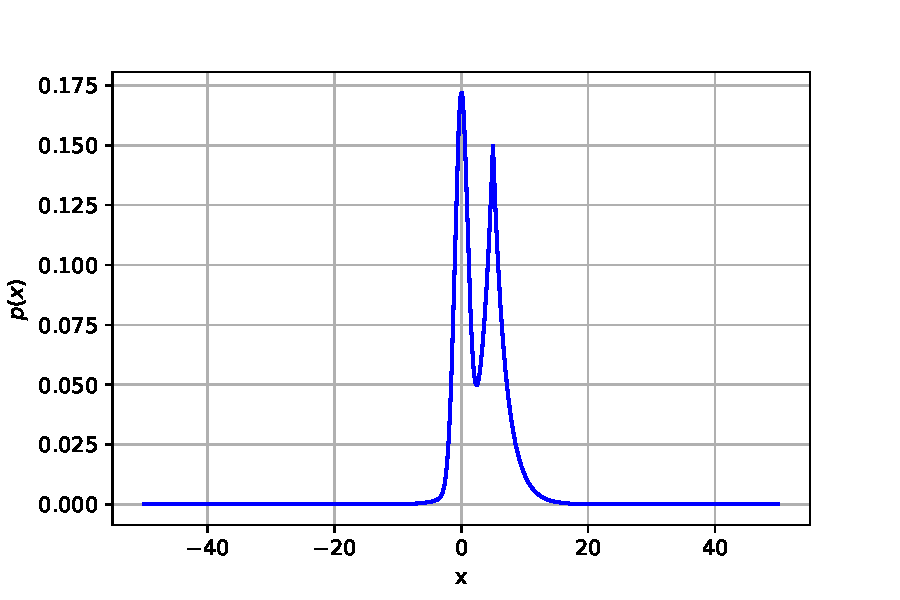
\includegraphics[scale=0.6]{Q1a.pdf}
		\caption{The distribution in Equation \eqref{eq:Q1_distribution} visualised over $x \in [-50, 50]$.}
		\label{fig:Q1_distribution}
	\end{figure}
	
	To test whether the distribution of interest is valid, we need to consider the properties that constitute a valid distribution. These properties are 
	\begin{enumerate}
		\item $p(x) \geq 0$, $\forall x$.
		\item $\int_{x} p(x) dx = 1$.
	\end{enumerate}

	The first property is resolved as both the Laplacian and Gaussian distributions in Equation \eqref{eq:Q1_distribution} are nonnegative $\forall$ $x$, and both scale coefficients $a_1$ and $a_2$ are non-negative. The second property is resolved as the integral of a linear combination of functions is a linear combination of function integrals. As such, the integral of interest becomes
	\begin{equation}
		\begin{aligned}
		\int_x p(x)dx &= \int_x (a_1 \cdot \mathcal{N}(x \vert 0, 1^2) + a_2 \cdot L(x \vert 5, 2)) dx\\
		&= a_1 \cdot \int_x \mathcal{N}(x \vert 0, 1^2)dx + a_2 \cdot \int_x L(x \vert 5, 2) dx \\
		&= a_1 \cdot 1 + a_2 \cdot 1 \\
		&= 1.
		\end{aligned}
	\end{equation}

	For this problem, the objective is to use rejection sampling to draw samples from the distribution shown in Equation \eqref{eq:Q1_distribution}. The goal in rejection sampling is to sample from a complex, possibly unnormalised, distribution $\tilde{p}(x)$ (which may or may not be normalised) using a simpler distribution $q(x)$. This simpler distribution is commonly referred to as the proposal distribution. The rejection sampling procedure is given through
	\begin{itemize}
		\item Initialise a proposal distribution $q(x)$.
		\item Define/find a scale $k$ such that $k \cdot q(x) > \tilde{p}(x)$ $\forall x$.
		\item Draw a sample $x_i \sim q(x)$.
		\item Evaluate $q(x_i)$ and $\tilde{p}(x_i)$.
		\item Sample from a uniform distribution $u_i \sim U[0, 1]$.
		\item Accept the sample if $\frac{\tilde{p}(x_i)}{k \cdot q(x_i)} > u_i$, reject otherwise (alternatively, if $\tilde{p}(x_i) > u_i \cdot k \cdot q(x_i)$).
		\item Repeat until a suitable number of samples is drawn.
	\end{itemize}

	To proceed with rejection sampling, the goal is to explore the influence of \emph{i)} different proposal distributions,\emph{ii)} different parametrisations of the proposal distributions, and \emph{iii)} the effect of the scale parameter $k$ on the efficiency of the rejection sampling procedure. In the implementation of rejection sampling on this one-dimensional, the parameter $k$ can be resolved automatically by evaluating $k \cdot q(x) > \tilde{p}(x)$ $\forall x$ over an $x$-domain of interest, provided the domain is sufficiently diverse. The considered proposal distributions are the Gaussian distribution, the Laplacian distribution and Student's t distribution. A two degree of freedom t distribution is used for all experiments. The variance of the proposal distribution is of interest in this investigation, as this can greatly affect the efficiency of the rejection sampling process. To absolve any implementation ambiguity, it is assumed that the expectation $\mathbb{E}_{x \sim p(x)} \{ x\}$ is known. This is trivial to evaluate as it reduces to $\mathbb{E}_{x \sim p(x)} \{ x\} = a_1 \cdot \mu_{gauss} + a_2 \cdot \mu_{laplace} = 3$.
	
	In Figure \ref{fig:Q1_rejection_sampling_dists} the results of this investigation is shown. Figure \ref{fig:Q1_rejection_sampling_dists} clearly shows that the efficiency of rejection sampling, for the proposal distributions considered, is heavily reliant on the scale parameter $k$. Regardless of the parametrisation, there is an exponential decay in the efficiency as $k$ is increased. The best performing proposal distribution is the Student's t distribution with a location of 3 and a scale parameter of 5, which had an efficiency just over $30\%$. In Figure \ref{fig:Q1_rejection_sampling_dists}, the degradation of the efficiency as a function of an increasing scale parameter is crucial to highlight that distributions that are tight around $p(x)$ are crucial to improved efficiencies. This follows from the rejection sampling algorithm, as if the ratio $\frac{\tilde{p}(x_i)}{k \cdot q(x_i)}$ for any proposal distribution sample $x_i \sim q(x)$ is far from 1 and closer to zero (i.e., the scaled proposal distribution has high sample likelihood while the true distribution does not and vice versa), then more samples will be rejected. Hence, a tight proposal distribution is key to efficient rejection sampling.
	\begin{figure}[htb!]
		\centering
		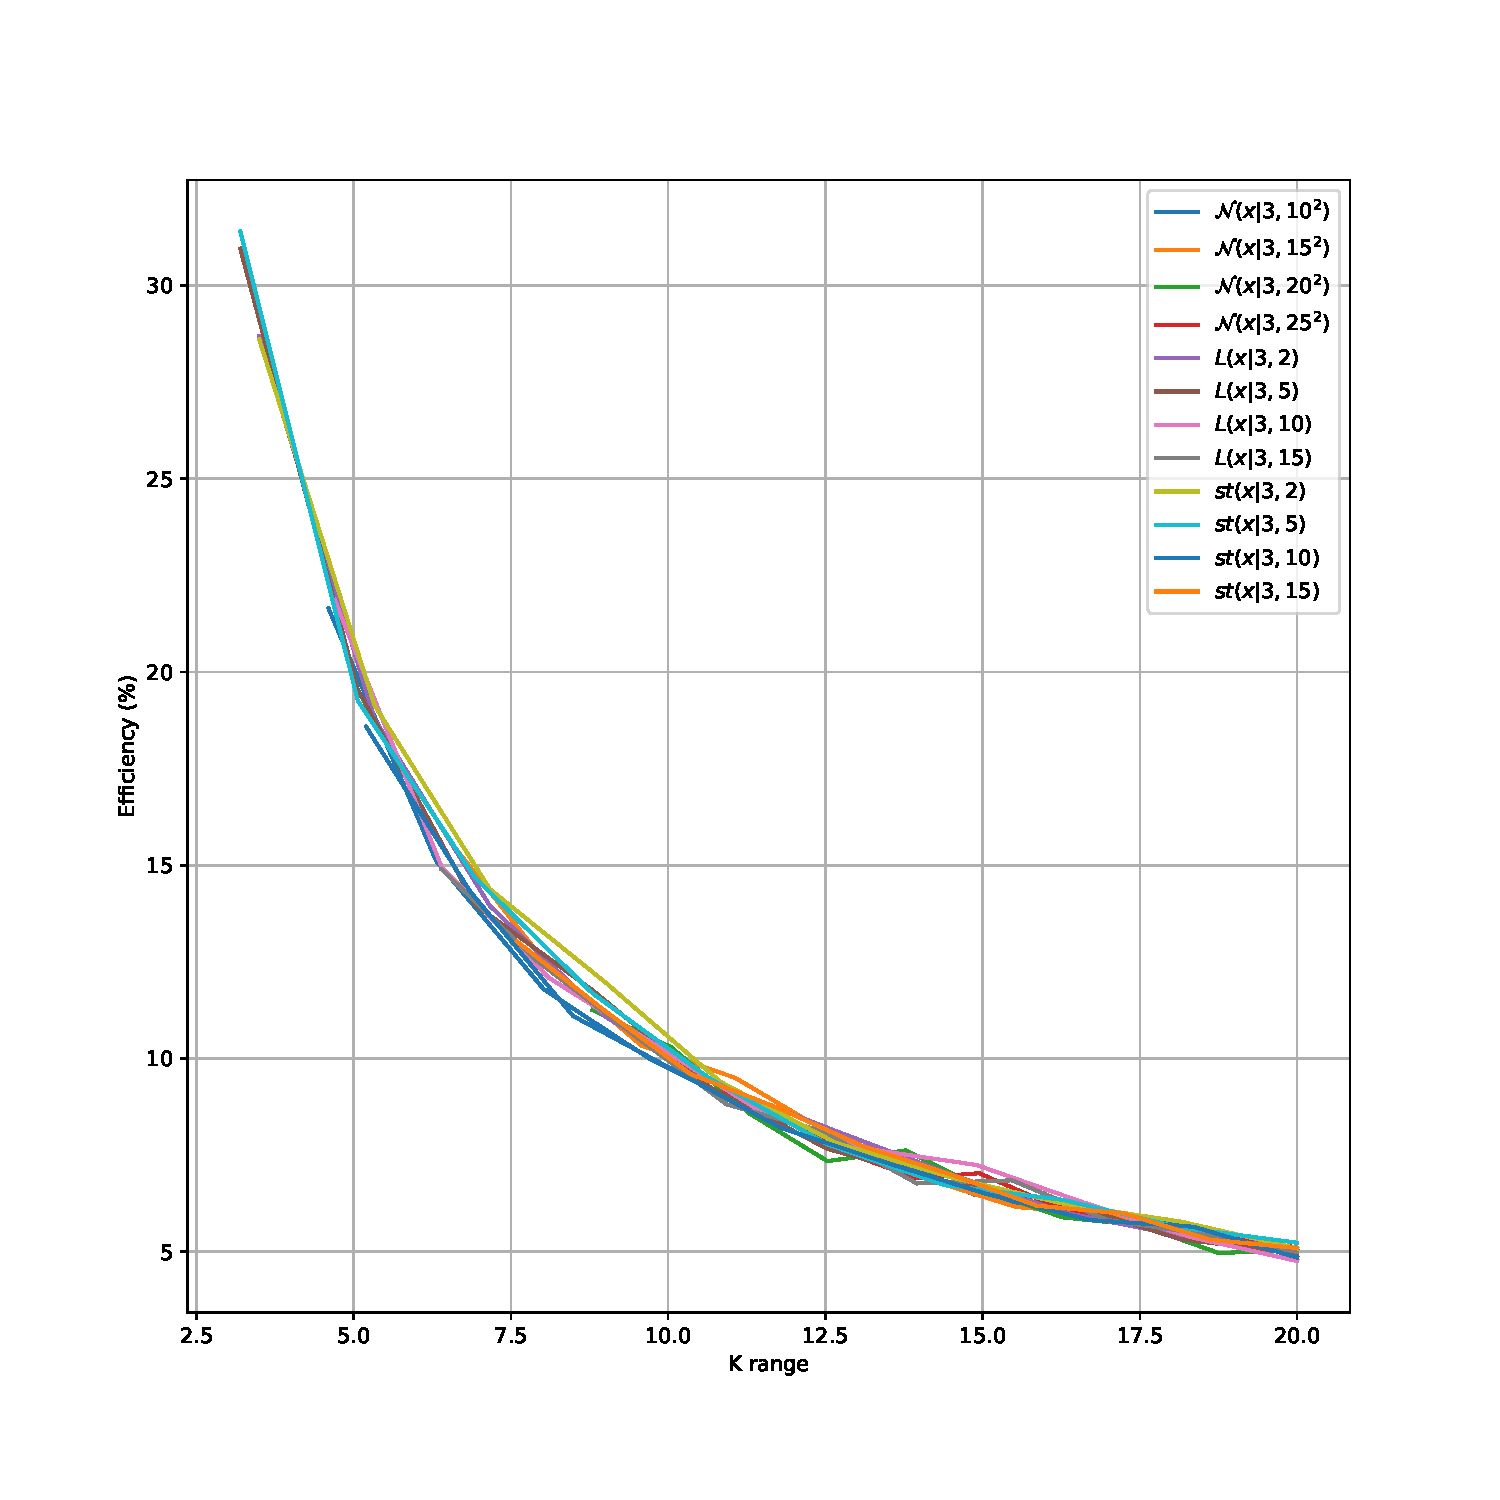
\includegraphics[scale=0.5]{Q1c.pdf}
		\caption{The efficiency of the rejection sampling procedure for 1000 samples under different parametrisations of the proposal distribution $q(x)$. Note that as the scale parameter $k$ was determined automatically, the starting points for each of the different distributions is not consistent.}
		\label{fig:Q1_rejection_sampling_dists}
	\end{figure}

	In Figure \ref{fig:Q1_rejection_sampling_samples}, the samples from the proposal distribution with the highest sampling efficiency are shown. It is clear that the rejection sampling process can correctly sample from $p(x)$. Now that samples from $p(x)$ may be drawn, the samples may be used to inspect different aspects of $p(x)$. 
	\begin{figure}[htb!]
		\centering
		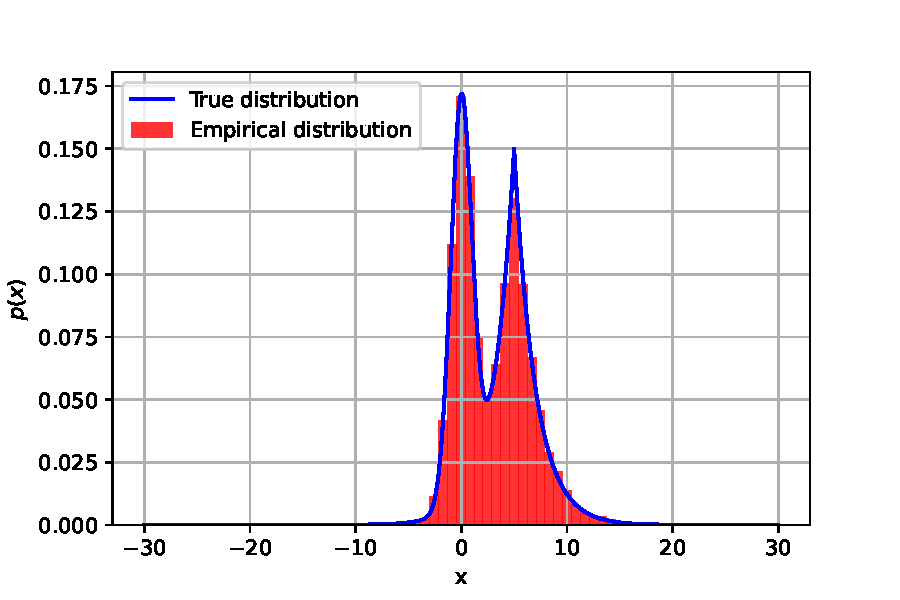
\includegraphics[scale=0.7]{Q1c_2.pdf}
		\caption{The samples from $p(x)$ using rejection sampling and a proposal distribution $\text{st}_{2}(x \vert 3, 5)$. }
		\label{fig:Q1_rejection_sampling_samples}
	\end{figure}

	The aspects of interest for this problem are:
	\begin{itemize}
		\item $\mathbb{E}_{x \sim p(x)} \{ x^2 \} = \int_x x^2 p(x)dx$.
		\item $P(x > 5) = \mathbb{E}_{x \sim p(x)} \{ I(x \vert -\infty, 5) \} = \int_x p(x)I(x \vert \infty, 5)dx$.
		\item The $3^{rd}$ percentile of $p(x)$. 
	\end{itemize}
	
	Note that $I(x \vert -\infty, 5)$ is an indicator function defined through
	\begin{equation}
		I(x \vert a, b) = \begin{cases} 
			1 & \text{if }  a \leq x \leq b, \\
			0 & \text{otherwise,}
		\end{cases}.
	\end{equation}

	To estimate the aspects of interest, Monte Carlo integration was used. To compare the performance of the estimates obtained through Monte Carlo integration, numerical integration was used to evaluate the aspects analytically. In Table \ref{tab:Q1_estimates} the results for the two estimation methods are shown. It is clear that the largest disparity in Table \ref{tab:Q1_estimates} was for the $\mathbb{E}_{x \sim p(x)} \{ x^2 \}$ estimate. The remaining estimates are numerically close, which indicates that the error in the $\mathbb{E}_{x \sim p(x)} \{ x^2 \}$ estimate may be resolved through sampling $p(x)$ more densely.
	\begin{table}[htb!]
		\centering
		\caption{The estimates of interest using the samples of $p(x)$ obtained using rejection sampling.}
		\label{tab:Q1_estimates}
		\begin{tabular}{@{}cccc@{}}
			\toprule
			Method               & $\mathbb{E}_{x \sim p(x)} \{x^2\}$ & $P(x > 5)$ & $3^{rd}$ percentile \\ \midrule
			Rejection sampling   & 20.527                            & 0.3037     & -1.6204         \\
			Numerical evaluation & 20.12                              & 0.3        & -1.6216        \\ \bottomrule
		\end{tabular}
	\end{table}

	To quantify the effect of the number of samples on the accuracy of the aforementioned estimates, Figure \ref{fig:Q1_estimate_error} was developed by evaluating the estimates as a function of the number of samples. It is clear that as the number of samples increases, the error in the Monte Carlo integration estimates decreases. This correctly suggests that in order to obtain an accurate Monte Carlo estimate, a large number of samples must be used. 
	\begin{figure}[htb!]
		\centering
		\begin{subfigure}[b]{0.45\textwidth}
			\centering
			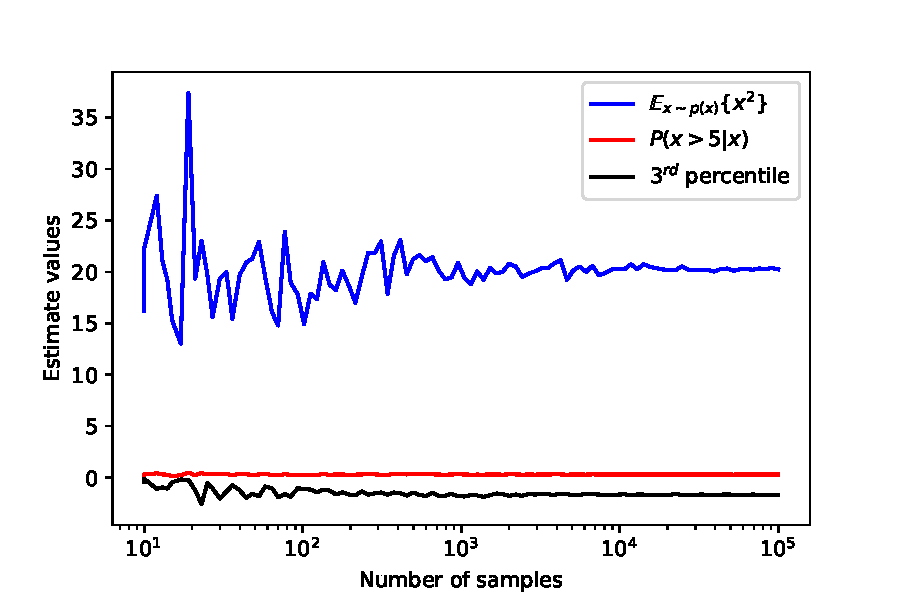
\includegraphics[width=\textwidth]{Q1g_1.pdf}
			\caption{The estimate-sample dependency.}
		\end{subfigure}
		~
		\begin{subfigure}[b]{0.45\textwidth}
			\centering
			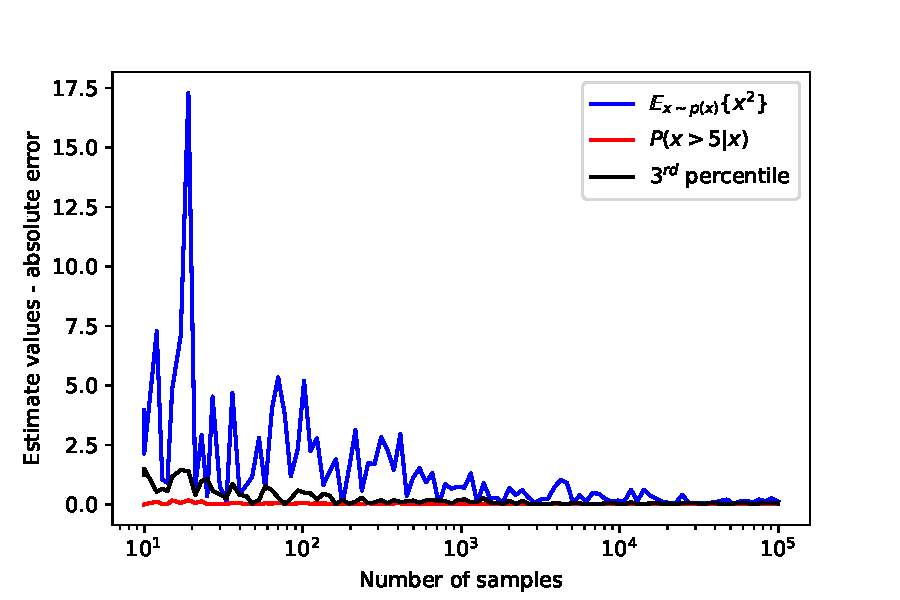
\includegraphics[width=\textwidth]{Q1g_2.pdf}
			\caption{The estimate-sample error.}
		\end{subfigure}
		
		\caption{The effect of the number of samples on the estimates. (a) shows the variation in the estimate and (b) shows the estimate error as a function of the number of samples. Note that the estimates were obtained as a once-off result, and as such this figure does not effectively convey the variation in the estimates for a given number of samples. However, it is clear that increasing the number of samples reduces the error in the estimates.}
		\label{fig:Q1_estimate_error}
	\end{figure}
	
	\clearpage
	
	\section{Question 2}
	
	Consider the generative model
	\begin{equation}
		x_n = \theta + \epsilon_n,
	\end{equation}
	where $\epsilon_n$ is a Laplacian distribution with a known scale parameter of $2$ and a location of $0$, $\epsilon \sim L(\epsilon \vert 0, 2)$. The population parameter $\theta$ is three and not known during the inference process. The following measured data is available for this problem:
	\begin{equation}
		\begin{aligned}
		\mathbf{x} = &[4.171206 , 3.06754327, 2.16931111, 2.00839214, 4.10014516, \\
		& 3.51408053, 2.86609886, 6.3492669 , 2.90566741, 5.99086803]^T
		\end{aligned}
	\end{equation}
	
	The objective of this problem is to use Markov Chain Monte Carlo (MCMC) to sample from the posterior distribution over the unknown parameter. The MCMC method in this problem uses the Metropolis-Hastings algorithm, and may be given as
	\begin{enumerate}
		\item Assume the proposal distribution $q(\theta)$, the unnormalised distribution of interest $\tilde{p}(\theta)$, a starting point $\theta_0$, and the number of iterations $N$.
		\item For $n = 1, \cdots, N$:
		\begin{itemize}
			\item Sample from the proposal distribution $\theta_{n} \sim q(\theta \vert \theta_{n - 1})$
			\item Draw a random sample $u_i \sim U[0, 1]$
			\item Accept the $\theta_n$ sample if $\min \left( 1, \frac{\tilde{p}(\theta_{n}) q(\theta_{n - 1} \vert \theta_{n}) }{\tilde{p}(\theta_{n - 1}) q(\theta_{n} \vert \theta_{n - 1})} \right) \geq u_i$, reject otherwise
			\item If reject: $\theta_{n} = \theta_{n - 1}$
			\item If accept: $\theta_{n}$ is kept
		\end{itemize}
	\end{enumerate}

	Once the samples have been obtained using a MCMC method, the goal is to determine some expectations and probabilities that are of interest for this problem. The elements of interest, which are to be found using Monte Carlo integration, are
	\begin{itemize}
		\item $\mathbb{E}_{\theta \sim p(\theta \vert \mathbf{x})} \{ \theta^2 \}$.
		\item $P(\theta > 3 \vert \mathbf{x})$.
		\item $P(x > 3 \vert \mathbf{x})$.
	\end{itemize}

	It is important to note that $P(x > 3 \vert \mathbf{x})$ is equal to  
	\begin{equation}
		P(x > 3 \vert \mathbf{x})= 1 - \mathbb{E}_{x \sim p(x \vert \mathbf{x})} \{ I(x \vert -\infty, 3) \}
	\end{equation} 
	which requires access to samples from $p(x \vert \mathbf{x})$. To obtain posterior predictive distribution samples, $\theta$ samples may be drawn from the posterior distribution $\theta_i \sim p(\theta \vert \mathbf{x})$, and a corresponding set of generative model samples $x \sim p(x \vert \theta_i)$ can then be drawn. The expectation of interest may then be determined for each $\theta_i$ sample and the average of these expectations is used to approximate $\mathbb{E}_{x \sim p(x \vert \mathbf{x})} \{ I(x, -\infty, 3) \}$. 
	
	The parameters of the proposal distribution are critical to the performance of the MCMC algorithm. To establish how the MCMC algorithm depends on the proposal distribution and the parameters therein, a investigation must occur. As such, a Laplacian and Gaussian proposal distribution will be used and the variance of these distributions will be changed. To determine the effects of the proposal distribution on the MCMC algorithm, the acceptance ratio and the aforementioned estimates will be tracked. The next objective is to describe the distributions of interest.
	
	The prior used in this problem is a Gaussian prior with a mean of 0 and a variance of 25. The distributions of interest here are the prior, the generative model which produces the likelihood function, and the unnormalised posterior. Mathematically, the prior is given as
	\begin{equation}
		\begin{aligned}
			p(\theta) &= \mathcal{N}(\theta \vert \theta_0, \sigma_0^2) \\
			&= \frac{1}{\sqrt{2 \cdot \pi \cdot \sigma_0^2}} \exp \left( -\frac{1}{2 \cdot \sigma_0^2} \cdot \left( \theta - \theta_0 \right)^2 \right),
		\end{aligned}
	\end{equation}
	where $\theta_0 = 0$ and $\sigma_0 = 5$. The generative model
	\begin{equation}
		\begin{aligned}
			p(x \vert \theta) = L(x \vert \theta, b)
			&= \frac{1}{2 \cdot b} \cdot \exp \left( -\frac{\vert x - \theta \vert}{b} \right),
		\end{aligned}
	\end{equation}
	gives rise to the likelihood function
	\begin{equation}
		\begin{aligned}
			p(\mathbf{x} \vert \theta) &= \prod_{n=1}^{N} p(x_n \vert \theta) \\
			\mathcal{L}(\theta \vert \mathbf{x}, b) &= \prod_{n=1}^{N} \frac{1}{2 \cdot b} \cdot \exp \left( -\frac{\vert x_n - \theta \vert}{b} \right),
		\end{aligned}
	\end{equation}
	
	Finally, the unnormalised posterior is given through
	\begin{equation}\label{eq:unnormalised_posterior}
		\begin{aligned}
			p(\theta, \mathbf{x}) &= p(\mathbf{x} \vert \theta) p(\theta) \\
			F(\theta \vert \theta_0, \sigma_0, \mathbf{x}, b) &=  \frac{1}{\sqrt{2 \cdot \pi \cdot \sigma_0^2}} \exp \left( -\frac{1}{2 \cdot \sigma_0^2} \cdot \left( \theta - \theta_0 \right)^2 \right) \prod_{n=1}^{N} \frac{1}{2 \cdot b} \cdot \exp \left( -\frac{\vert x_n - \theta \vert}{b} \right),
		\end{aligned}
	\end{equation}

	It is important to note here that the goal is to draw samples from the posterior using MCMC. Thus, the distribution of interest $\tilde{p}(\theta)$ is the unnormalised posterior given in Equation \eqref{eq:unnormalised_posterior}. In Figure \ref{fig:Q2_distributions}, the prior and unnormalised posterior distributions alongside the likelihood function is shown. 
	\begin{figure}[htb!]
		\centering
		\begin{subfigure}[b]{0.45\textwidth}
			\centering
			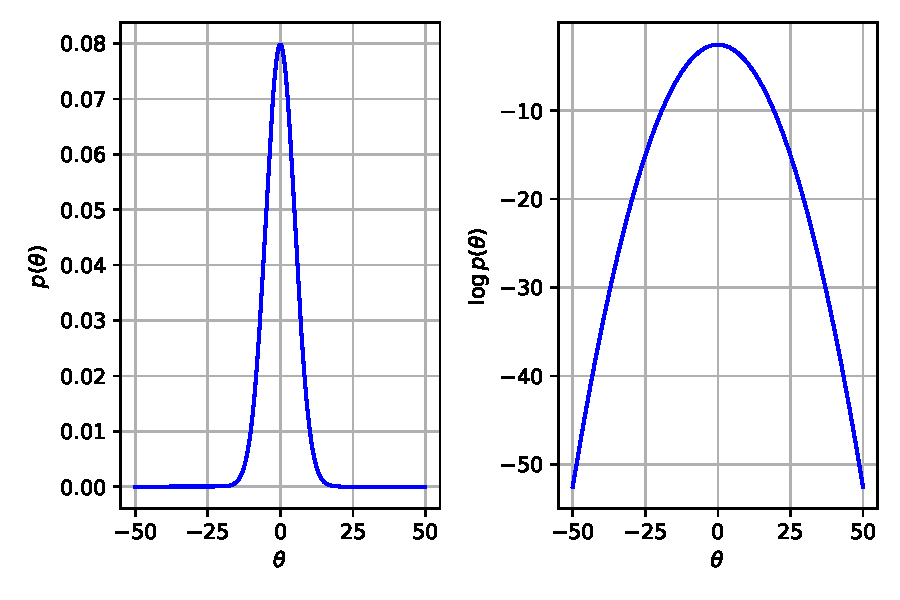
\includegraphics[width=\textwidth]{Q2b_1.pdf}
			\caption{The prior.}
		\end{subfigure}
		~
		\begin{subfigure}[b]{0.45\textwidth}
			\centering
			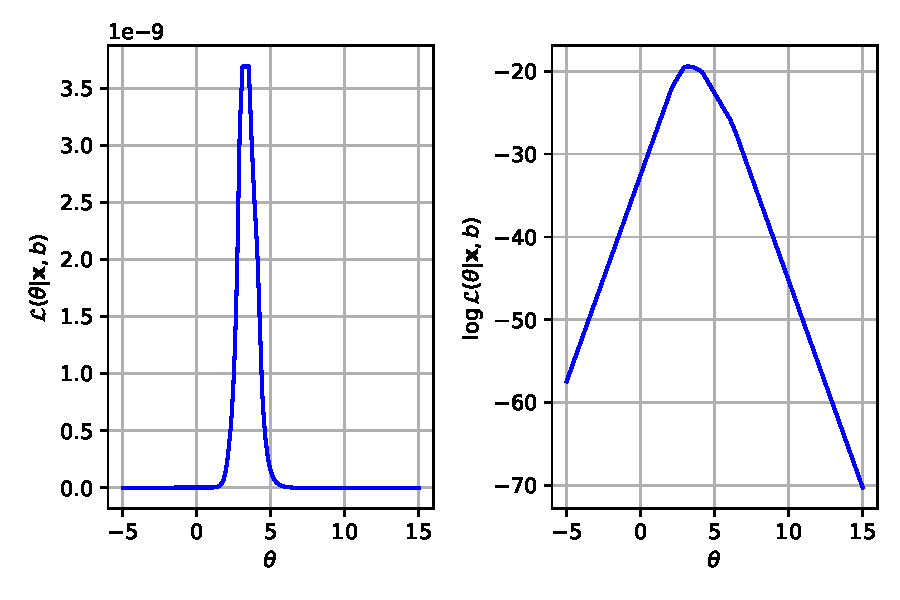
\includegraphics[width=\textwidth]{Q2b_2.pdf}
			\caption{The likelihood function.}
		\end{subfigure}
	
		\begin{subfigure}[b]{0.45\textwidth}
			\centering
			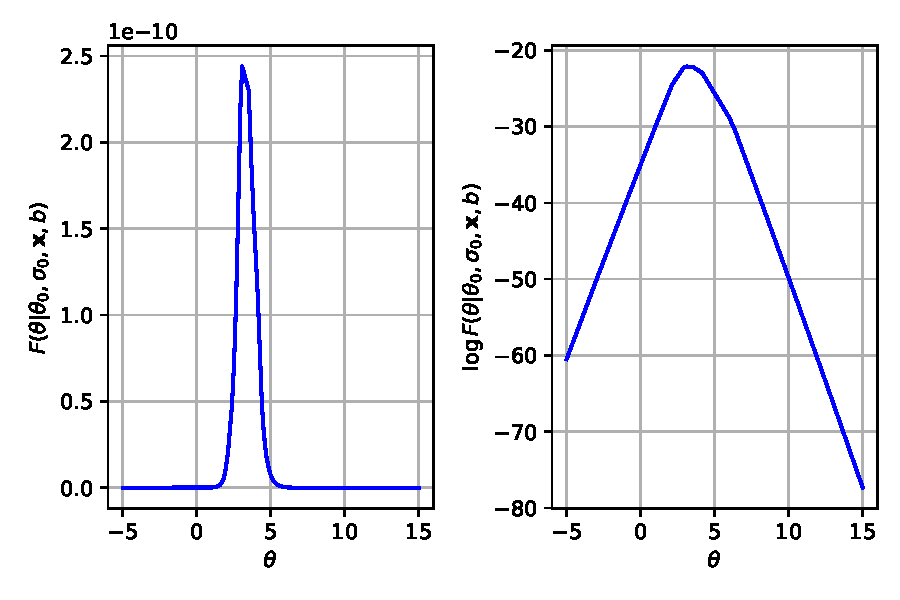
\includegraphics[width=\textwidth]{Q2b_3.pdf}
			\caption{The unnormalised posterior.}
		\end{subfigure}
		
		\caption{The prior, likelihood function and the unnormalised posterior for the second problem.}
		\label{fig:Q2_distributions}
	\end{figure}

	In Table \ref{tab:Q2_results}, the results of the MCMC method for different proposal distributions is shown. Crucially, it is seen that as the variance of the proposal distribution increased, the acceptance ratio subsequently decreased. This is beneficial to the MCMC method as a highly localised variance biases the method to only accept samples if the distribution of interest increases in likelihood, whereas a lower variance encourages the model to explore the parameter space and obtain better samples. The clear correlation to the proposal distribution variance indicates that a better change of accepting a new sample if the proposal distribution is highly localised. However, the danger of a high acceptance ratio is that there is no guarantee that you are exploring the space, you only know that you are increasing the likelihood ratio $\frac{\tilde{p}(\theta_n)}{\tilde{p}(\theta_{n - 1})}$. Alternatively, a low acceptance ratio may indicate that the exploration has gone off course, and hence you are sampling from regions where $\tilde{p}(\theta)$ does not lie. Thus, there is a natural trade-off between improving the parameter space likelihood improvement and exploration. 
	\begin{table}[htb!]
		\centering
		\caption{The acceptance ratio and the estimates of interest for different proposal distributions with different initial parameters. Note that the estimates do not effectively capture the variation in the value of the estimates, and hence are biased as they were determined once off. A tuning period of $50\%$, a thinning size of 10, and 100 000 iterations were performed for all experiments.}
		\label{tab:Q2_results}
		\begin{tabular}{@{}ccccc@{}}
			\toprule
			Proposal distribution & Acceptance ratio & $\mathbb{E}_{\theta \sim p(\theta \vert \mathbf{x})} \{\theta^2\}$ & $P(\theta > 3 \vert \mathbf{x})$ & $P(x > 3 \vert \mathbf{x})$ \\ \midrule
			Gaussian ($N(\theta \vert 0, 0.25^2)$ & $86.43 \%$ & 11.7337 & 0.7314 & 0.5742 \\
			Laplacian $L(\theta \vert 0, 0.25)$ & $83.41 \%$ & 11.6734 & 0.7342 & 0.5725 \\
			Gaussian ($N(\theta \vert 0, 0.5^2)$ & $73.31 \%$ & 11.823 & 0.731 & 0.5759 \\
			Laplacian $L(\theta \vert 0, 0.5)$ & $69.77 \%$ & 11.7571 & 0.7368 & 0.5751 \\
			Gaussian ($N(\theta \vert 0, 2^2)$ & $33.40 \%$ & 11.8197 & 0.7378 & 0.5754 \\
			Laplacian $L(\theta \vert 0, 2)$ & $33.2 \%$ & 11.7278 & 0.7272 & 0.5730 \\
			Gaussian ($N(\theta \vert 0, 2^2)$ & $14.68 \%$ & 11.6620 & 0.722 & 0.5712 \\
			Laplacian $L(\theta \vert 0, 2)$ & $15.88 \%$ & 11.6514 & 0.7314 & 0.5714 \\ \bottomrule
		\end{tabular}
	\end{table}

	Finally, it is important to quantify the effect of the number of samples on the accuracy of the aforementioned estimates. Figure \ref{fig:Q1_estimate_error} was developed by evaluating the estimates as a function of the number of samples. It is clear that as the number of samples increases, the error in the Monte Carlo integration step of the MCMC sample estimates decreases. This correctly suggests that in order to obtain an accurate Monte Carlo estimate, a large number of samples must be used. 
	\begin{figure}[htb!]
		\centering
		\begin{subfigure}[b]{0.45\textwidth}
			\centering
			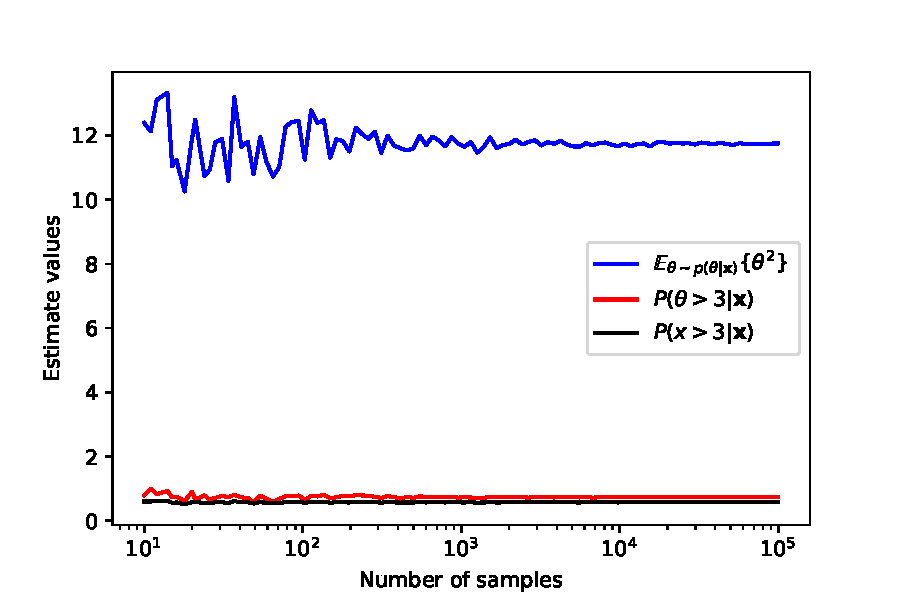
\includegraphics[width=\textwidth]{Q2g_1.pdf}
			\caption{The estimate-sample dependency.}
		\end{subfigure}
		~
		\begin{subfigure}[b]{0.45\textwidth}
			\centering
			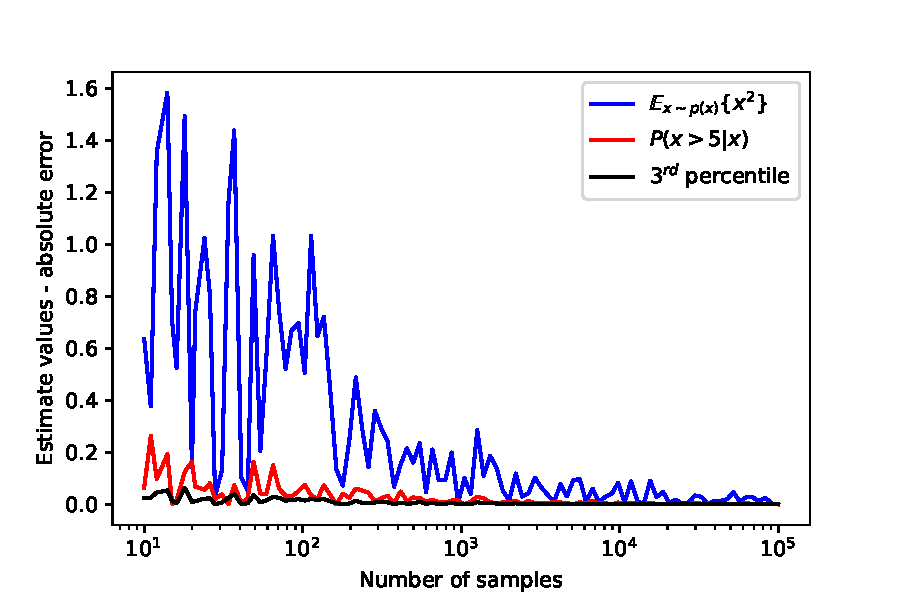
\includegraphics[width=\textwidth]{Q2g_2.pdf}
			\caption{The estimate-sample error.}
		\end{subfigure}
		
		\caption{The effect of the number of samples on the MCMC-based estimates. (a) shows the variation in the estimate and (b) shows the estimate error as a function of the number of samples. Note that the estimates were obtained as a once-off result, and as such this figure does not effectively convey the variation in the estimates for a given number of samples. However, it is clear that increasing the number of samples reduces the error in the estimates. A Gaussian distribution with a mean of 0 and a variance of $2^2$ was used for all iterations.}
		\label{fig:Q2_estimate_error}
	\end{figure}
	
	\clearpage
	
	\section{Question 3}
	
	The objective of the third problem is to perform Bayesian inference on a linear elastic-linear hardening material model. The model of interest is given by
	\begin{equation}
		\sigma_{meas} = \sigma_l(\epsilon, \boldsymbol\theta) + \nu,
	\end{equation} 
	where $\epsilon$ is strain, $\boldsymbol\theta = [E, \sigma_{y_0}, H]^T$, $E$ is the Young's Modulus, $\sigma_{y_0}$ is the yield strength and $H$ is the plastic modulus. The additive noise $\nu$ is obtained from a zero-mean Gaussian with an unknown variance $\eta^2$. The material model $\sigma_l(\eta, \boldsymbol\theta)$ is given by
	\begin{equation}
		\sigma_l(\epsilon, \boldsymbol\theta) = E \cdot \epsilon \cdot \left( 1 - h(\epsilon - \frac{\sigma_{y_0}}{E}) \right) + \left( \sigma_{y_0} + \frac{H \cdot E}{H + E} \cdot \left[ \epsilon - \frac{\sigma_{y_0}}{E} \right] \right) \cdot h(\epsilon - \frac{\sigma_{y_0}}{E}),
	\end{equation}
	where $h(\cdot)$ is the heavyside function
	\begin{equation}
		h(x) = \begin{cases} 
			1 & \text{if }  x \geq 0, \\
			0 & \text{if } x \leq 0
		\end{cases}.
	\end{equation}

	To ensure that the model does not succumb to the units of the different parameters, the parameters are scaled as follows:
	\begin{itemize}
		\item $E = 10^{11} \cdot \tilde{E}$
		\item $\sigma_{y_0} = 10^{11} \cdot \tilde{\sigma}_{y_0}$
		\item $H = 10^{11} \cdot \tilde{H}$
	\end{itemize}
	where $\tilde{\boldsymbol\theta} = \left[ \tilde{E}, \tilde{\sigma}_{y_0}, \tilde{H} \right]$. The prior over the scaled parameters $\{\tilde{\boldsymbol\theta}, \eta \}$ is given as a factorial Gamma prior
	\begin{equation}
		p(\tilde{\boldsymbol\theta}, \eta) = \text{Ga} \left( \tilde{E}, \alpha = 3, \beta = 1 \right) \cdot \text{Ga} \left( \tilde{\sigma}_{y_0}, \alpha = 3, \beta = 1 \right) \cdot \text{Ga} \left( \tilde{H}, \alpha = 3, \beta = 1 \right) \cdot \text{Ga} \left( \eta, \alpha = 3, \beta = 1 \right).
	\end{equation}

	The goal is to use PyMC3 to sample from the posterior distribution, and then compare the posterior to a pre-defined Gaussian posterior distribution. The goal here is to ask questions about the material model given some observed data. The observed data in this question is shown in Figure \ref{fig:Q3_observed_data} superimposed over two initialisations of the material model with zero noise.
	\begin{figure}[htb!]
		\centering
		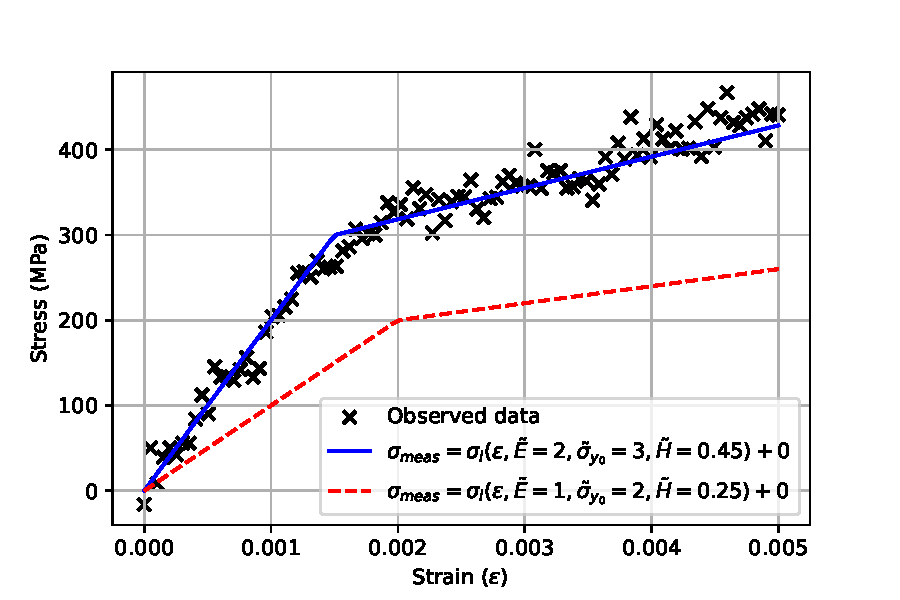
\includegraphics[scale=0.5]{Q3a.pdf}
		\caption{The observed material data for the third problem.}
		\label{fig:Q3_observed_data}
	\end{figure}

	\subsection{PyMC3 analysis}
	In the first part of this problem, the objective is to use \texttt{PyMC3} to sample from the posterior distribution. In Figure \ref{fig:Q3_pymc3_prior_post_samples} the samples from the prior and posterior distributions $p(\tilde{\boldsymbol\theta}, \eta)$ and $p(\tilde{\boldsymbol\theta}, \eta \vert \boldsymbol\sigma_{meas}, \boldsymbol\epsilon)$ are shown. The change in the parameters is distinct, as the posterior distributions are all less skewed. The MAP estimate of the model parameters was found to be $\{\boldsymbol\theta, \eta \}_{MAP} = \{E = 189.844 GPa, \sigma_{y_0} = 300.997MPa, H = 54.188GPa, \eta = 16.002  \}$. In Figure \ref{fig:Q3_pymc3_prior_post_predictive_samples} the prior and posterior distribution samples are used to draw samples from the prior and posterior predictive distributions. In Figure \ref{fig:Q3_pymc3_prior_post_predictive_PyMC3}, the \texttt{PyMC3} posterior predictive samples is shown. I suspect that PyMC3 follows the sample process to sample from the prior and posterior predictive distributions as was done in this work.
	\begin{figure}[htb!]
		\centering
		\begin{subfigure}[b]{0.45\textwidth}
			\centering
			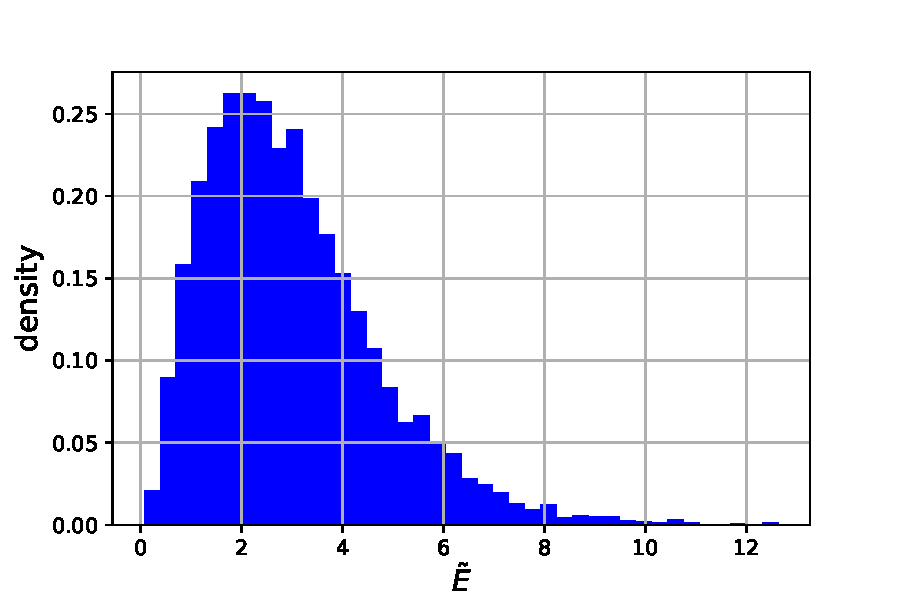
\includegraphics[width=\textwidth]{Q3a_1.pdf}
			\caption{Prior $\tilde{E}$ samples.}
		\end{subfigure}
		~
		\begin{subfigure}[b]{0.45\textwidth}
			\centering
			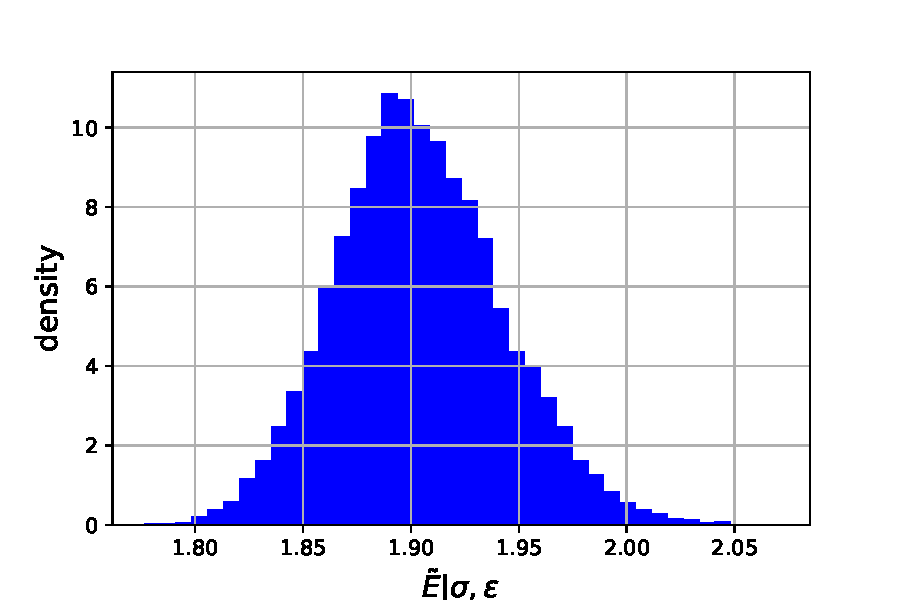
\includegraphics[width=\textwidth]{Q3a_6.pdf}
			\caption{Posterior $\tilde{E}$ samples.}
		\end{subfigure}
	
		\begin{subfigure}[b]{0.45\textwidth}
			\centering
			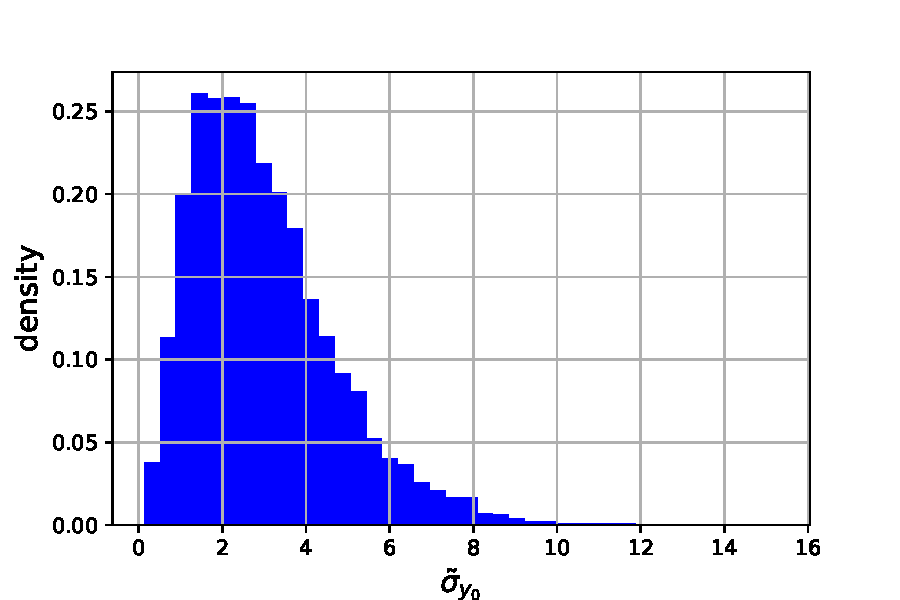
\includegraphics[width=\textwidth]{Q3a_2.pdf}
			\caption{Prior $\tilde{\sigma}_{y_0}$ samples.}
		\end{subfigure}
		~
		\begin{subfigure}[b]{0.45\textwidth}
			\centering
			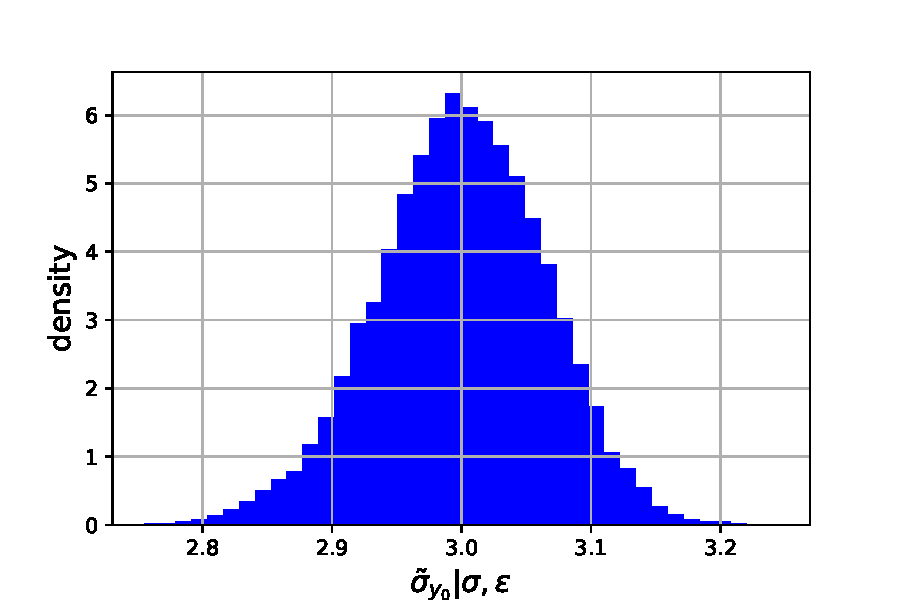
\includegraphics[width=\textwidth]{Q3a_7.pdf}
			\caption{Posterior $\tilde{\sigma}_{y_0}$ samples.}
		\end{subfigure}
	
		\begin{subfigure}[b]{0.45\textwidth}
			\centering
			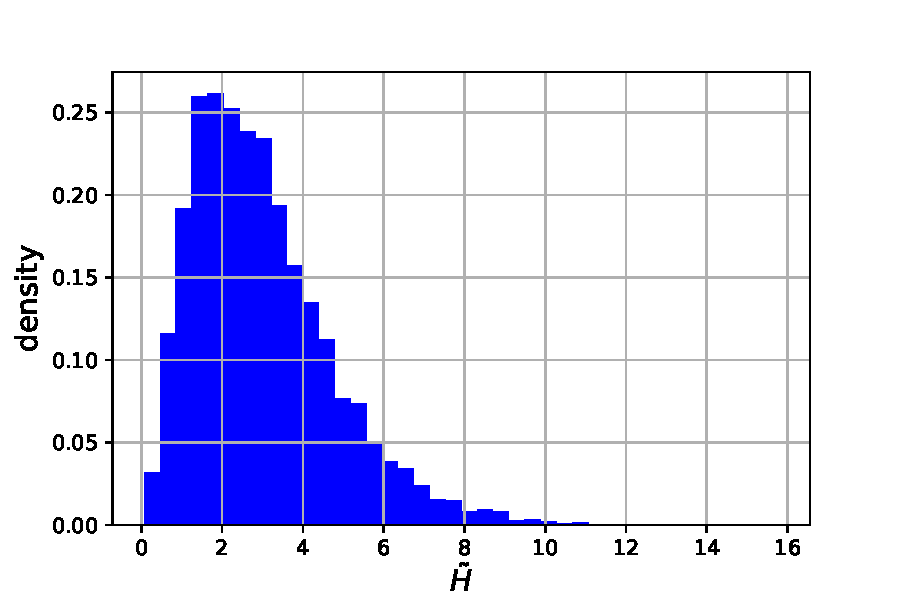
\includegraphics[width=\textwidth]{Q3a_3.pdf}
			\caption{Prior $\tilde{H}$ samples.}
		\end{subfigure}
		~
		\begin{subfigure}[b]{0.45\textwidth}
			\centering
			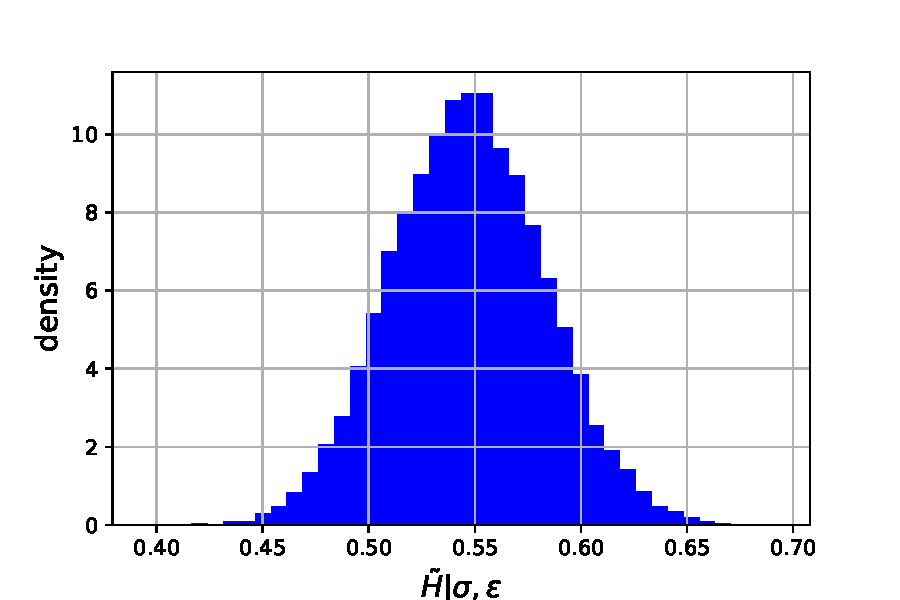
\includegraphics[width=\textwidth]{Q3a_8.pdf}
			\caption{Posterior $\tilde{H}$ samples.}
		\end{subfigure}
	
		\begin{subfigure}[b]{0.45\textwidth}
			\centering
			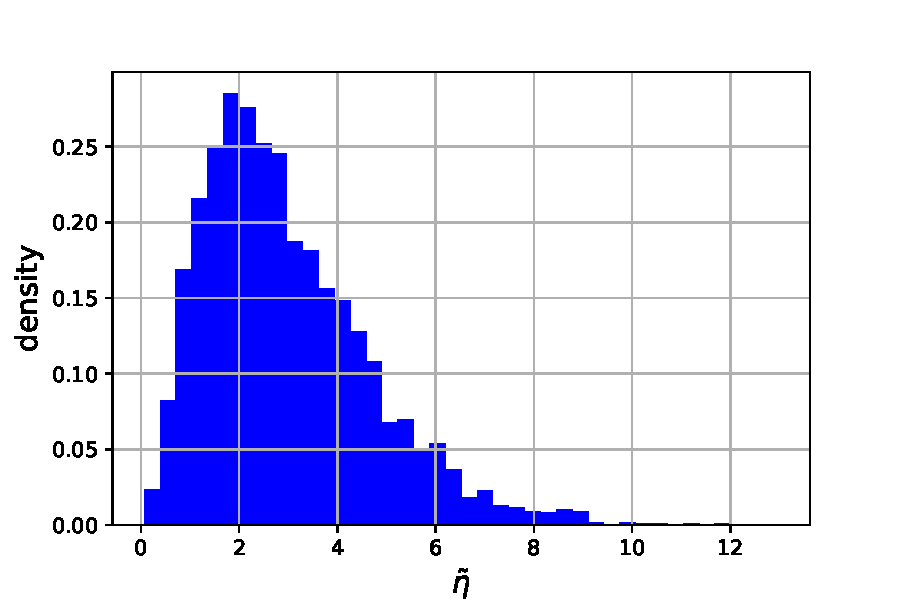
\includegraphics[width=\textwidth]{Q3a_4.pdf}
			\caption{Prior $\eta$ samples.}
		\end{subfigure}
		~
		\begin{subfigure}[b]{0.45\textwidth}
			\centering
			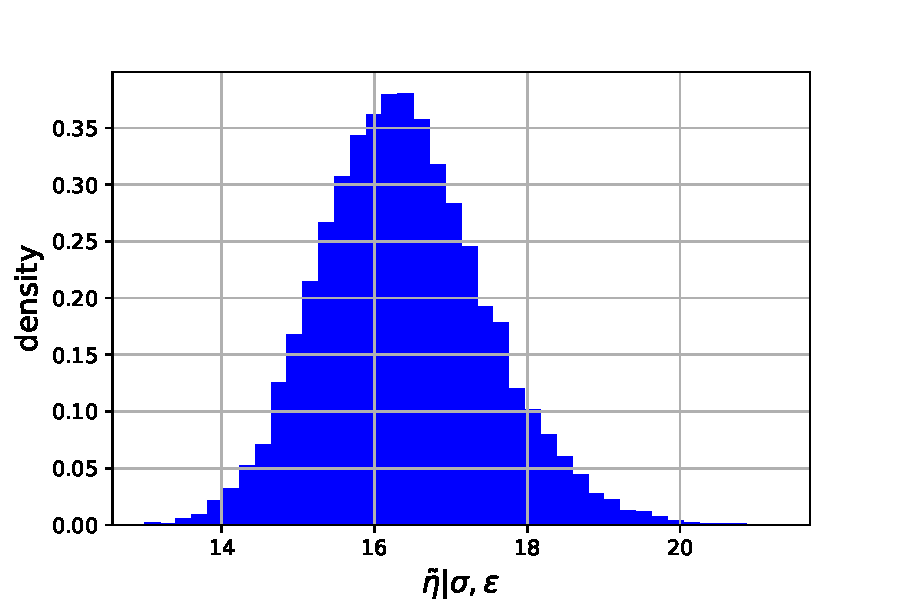
\includegraphics[width=\textwidth]{Q3a_9.pdf}
			\caption{Posterior $\eta$ samples.}
		\end{subfigure}
		
		\caption{Samples from the prior and posterior distributions over $\{\tilde{\boldsymbol\theta}, \eta\}$.}
		\label{fig:Q3_pymc3_prior_post_samples}
	\end{figure}

	\begin{figure}[htb!]
	\centering
	\begin{subfigure}[b]{0.45\textwidth}
		\centering
		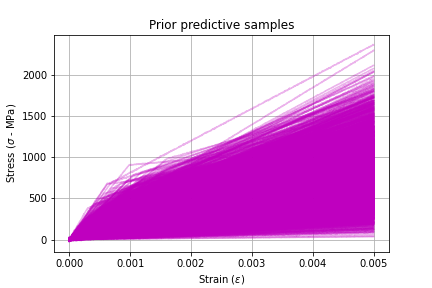
\includegraphics[width=\textwidth]{Q3a_5.png}
		\caption{Prior predictive distribution samples.}
	\end{subfigure}
	~
	\begin{subfigure}[b]{0.45\textwidth}
		\centering
		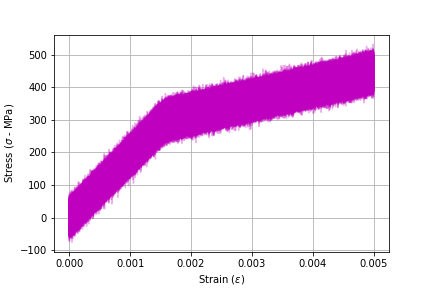
\includegraphics[width=\textwidth]{Q3a_10.png}
		\caption{Posterior predictive distribution samples.}
	\end{subfigure}
	
	\caption{Samples from the prior and posterior predictive distributions for the linear elasticity-linear hardening material model using the prior and posterior distribution \texttt{PyMC3} samples.}
	\label{fig:Q3_pymc3_prior_post_predictive_samples}
	\end{figure}

	\begin{figure}[htb!]
		\centering
		\begin{subfigure}[b]{0.45\textwidth}
			\centering
			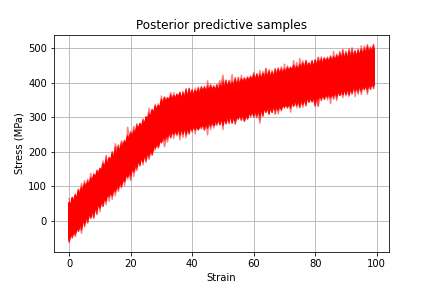
\includegraphics[width=\textwidth]{Q3a_11.png}
			\caption{Prior predictive distribution samples.}
		\end{subfigure}
		~
		\begin{subfigure}[b]{0.45\textwidth}
			\centering
			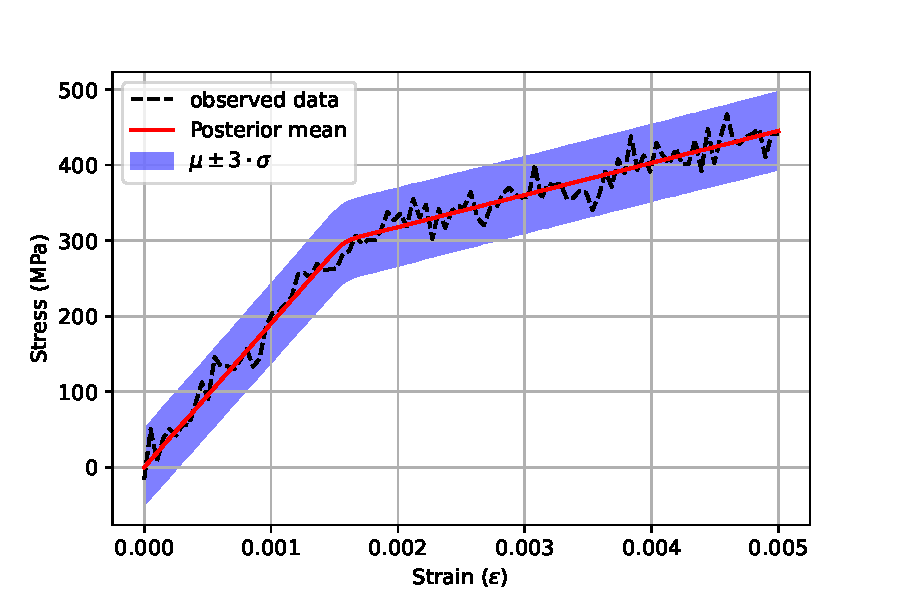
\includegraphics[width=\textwidth]{Q3a_12.pdf}
			\caption{Posterior predictive distribution samples.}
		\end{subfigure}
		
		\caption{Samples from the prior and posterior predictive distributions for the linear elasticity-linear hardening material model obtained using \texttt{PyMC3}.}
		\label{fig:Q3_pymc3_prior_post_predictive_PyMC3}
	\end{figure}

	Using the posterior samples the posterior mean and covariance was determined. This is given as
	\begin{equation}
	\boldsymbol\mu_{posterior} = \left[ 190400.157 MPa, 299.925MPa, 54681.867MPa, 16.39 \right]^T,
	\end{equation}
	\begin{equation}
		\boldsymbol\Sigma_{post} = \begin{bmatrix}
			1.501e^{7} & -1.228e^{4} & 1.778e^{6} & 0 \\
			-1.228e^{4} & 4.193e^{1} & -1.946e^{3} & 0 \\
			1.778e^{6} & -1.946e^{4} & 1.309e^{7} & 0 \\
			0 & 0 & 0 & 1 
		\end{bmatrix}.
	\end{equation}

	Finally, an investigation was performed into the effect of the prior hyper-parameters. In Figure \ref{fig:Q3_hyperparameter_effects} the influence of the $\alpha$ and $\beta$ terms in the priors on the posterior MAP estimate is shown. It is clear that model parameters are only sensitive to hyper-parameters where $\alpha \geq 9$ or $\beta \leq 0.5$. After these ranges, there is little noticeable variation in the MAP parameters.
	\begin{figure}[htb!]
		\centering
		\begin{subfigure}[b]{0.45\textwidth}
			\centering
			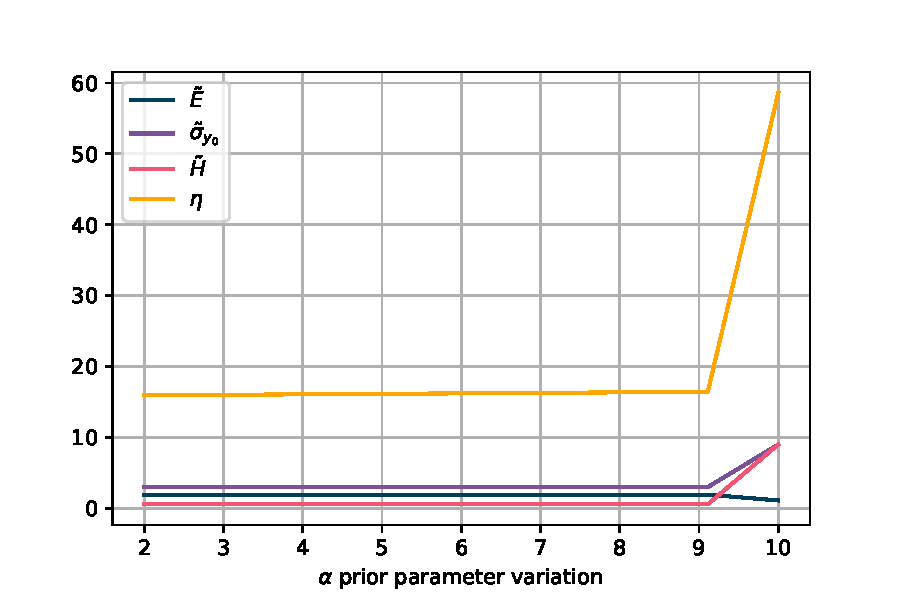
\includegraphics[width=\textwidth]{Q3a_13.pdf}
			\caption{$\alpha$ variation.}
		\end{subfigure}
		~
		\begin{subfigure}[b]{0.45\textwidth}
			\centering
			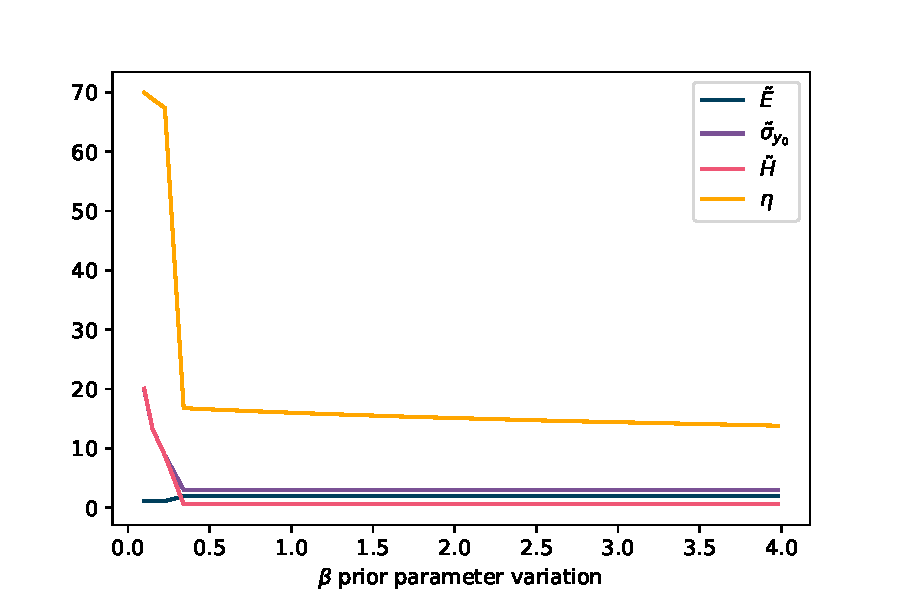
\includegraphics[width=\textwidth]{Q3a_14.pdf}
			\caption{$\beta$ variation.}
		\end{subfigure}
		
		\caption{The effect of the prior hyper-parameters on the MAP estimates of the model hyper-parameters.}
		\label{fig:Q3_hyperparameter_effects}
	\end{figure}
	
	\subsection{Application and inference}
	
	We can now use the results from \texttt{PyMC3} to answer questions about the model in this problem. To compare to the \texttt{PyMC3} results, a pre-defined posterior distribution is given as
	\begin{equation}\label{eq:predefined_posterior}
		p(\boldsymbol\theta, \eta \vert \boldsymbol\sigma_{meas}, \boldsymbol\epsilon) = \mathcal{N} \left( 
		\begin{bmatrix}
			E \\
			\sigma_{y_0} \\
			H \\
			eta 
		\end{bmatrix} \vert
		\begin{bmatrix}
			190 000 \\
			300 \\
			55 000 \\
			18 
		\end{bmatrix},
		\begin{bmatrix}
			2\cdot e^{7} & -1e^{-4} & 1e^{6} & 0 \\
			-1e^{-4} & 30 & -1e^{-4} & 0 \\
			1e^{6} & -1e^{4} & 1e^{7} & 0 \\
			0 & 0 & 0 & 1
		\end{bmatrix}
		 \right).
	\end{equation}

	Firstly, given an initial estimate of the model parameters $E = 200 GPa, \sigma_{y_0} = 300 MPa, H = 45 GPa$, we can determine the log-likelihood function as a function of $\eta$. This is possible as the generative model was assumed to be a Gaussian distribution
	\begin{equation}
		p(\sigma_{meas} \vert \sigma_l(\boldsymbol\theta, \epsilon), \eta) = \frac{1}{\sqrt{2\cdot \pi \cdot \eta^2}} \cdot \exp \left( -\frac{1}{2}\cdot \frac{\left( \sigma_{meas} - \sigma_l(\boldsymbol\theta, \epsilon) \right)^2}{\eta^2} \right).
	\end{equation}
	Hence, the log-likelihood function, given some observed data $\{\boldsymbol\sigma_{meas}, \boldsymbol\epsilon\}$, is given by
	\begin{equation}
		\begin{aligned}
			LL(\boldsymbol\theta, \eta \vert \boldsymbol\sigma_{meas}, \boldsymbol\epsilon) = -\frac{N}{2}\cdot \log(2 \cdot \pi) - \frac{N}{2}\cdot \log(\eta^2) - \frac{1}{2\cdot \eta^2}\sum_{n=1}^{N} \left[ \sigma_{meas, n} - \sigma_l(\boldsymbol\theta, \epsilon_n) \right]^2.
		\end{aligned}
	\end{equation}

	If the assumption is made that the noise $\eta$ is unknown, the resulting likelihood function is shown in Figure \ref{fig:Q3_noise_LL}. The parameter $\eta$ that maximised the likelihood function is $\eta = 19.023$. If the noise is known ($\eta = 18$), then the likelihood function evaluates to $LL(\boldsymbol\theta, \eta \vert \boldsymbol\sigma_{meas}, \boldsymbol\epsilon) = -437.307$ and the likelihood function evaluates to $L(\boldsymbol\theta, \eta \vert \boldsymbol\sigma_{meas}, \boldsymbol\epsilon) = 1.2022e^{-190}$.
	\begin{figure}[htb!]
		\centering
		\begin{subfigure}[b]{0.45\textwidth}
			\centering
			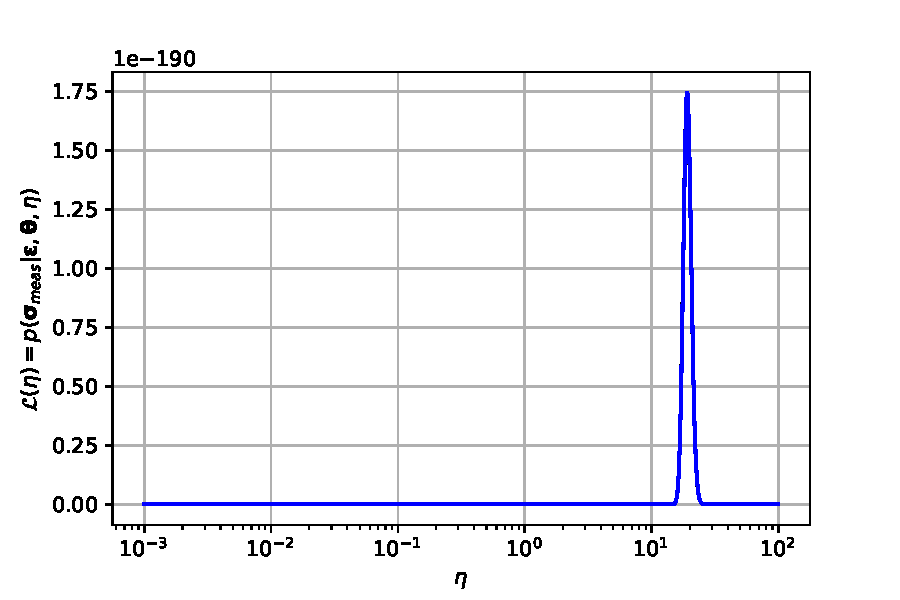
\includegraphics[width=\textwidth]{Q3b_2.pdf}
			\caption{Likelihood function over $\eta$.}
		\end{subfigure}
		~
		\begin{subfigure}[b]{0.45\textwidth}
			\centering
			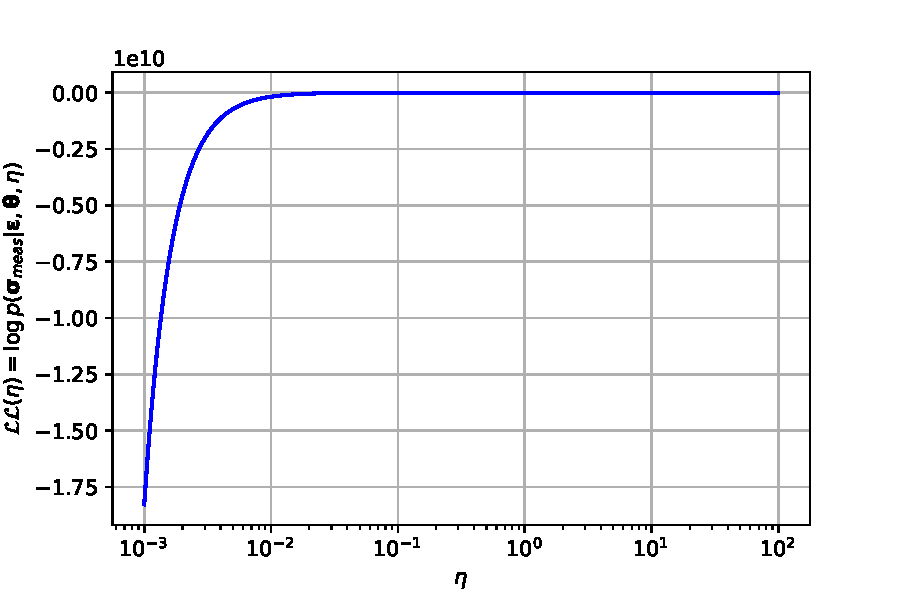
\includegraphics[width=\textwidth]{Q3b_1.pdf}
			\caption{Log-likelihood function over $\eta$.}
		\end{subfigure}
		
		\caption{The likelihood and log-likelihood function for $E = 200 GPa, \sigma_{y_0} = 300 MPa, H = 45 GPa$ and an unknown noise.}
		\label{fig:Q3_noise_LL}
	\end{figure}

	The next question of interest is: \emph{what is the $95\%$ credible interval for the posterior yield stress?} In this setting, the objective is to evaluate
	\begin{equation}
		\nu_{\alpha/2} \leq \sigma_{y_0} \vert \boldsymbol\sigma_{meas}, \boldsymbol\epsilon \leq \nu_{1 - \alpha/2},
	\end{equation}
	where $\alpha$ is the interval probability and $\nu_k$ is the $k^{th}$ percentile. This interval was found using samples from the posterior using the posterior given in Equation \eqref{eq:predefined_posterior} and \texttt{PyMC3}. These are given as
	\begin{equation}
		\text{Pre-defined posterior samples: } 289.274 \text{ MPa} \leq \sigma_{y_0} \vert \boldsymbol\sigma_{meas}, \boldsymbol\epsilon \leq 310.702 \text{ MPa},
	\end{equation}
	\begin{equation}
		\text{\texttt{PyMC3} posterior samples: } 286.801 \text{ MPa} \leq \sigma_{y_0} \vert \boldsymbol\sigma_{meas}, \boldsymbol\epsilon \leq 312.087  \text{ MPa},
	\end{equation}
	\clearpage
	
	The third question is: \emph{what is the expectation $\mathbb{E} \{  H \vert \boldsymbol\sigma_{meas}, \boldsymbol\epsilon \}$?} This can be found using Monte Carlo integration for samples from the posterior marginal distribution $p(H \vert \boldsymbol\sigma_{meas}, \boldsymbol\epsilon)$. Using the predefined posterior and the \texttt{PyMC3} samples, this evaluates to
	\begin{itemize}
		\item $\mathbb{E} \{  H \vert \boldsymbol\sigma_{meas}, \boldsymbol\epsilon \}_{pre-defined} = 54.987$ GPa
		\item $\mathbb{E} \{  H \vert \boldsymbol\sigma_{meas}, \boldsymbol\epsilon \}_{\texttt{PyMC3}} = 54.592$ GPa
	\end{itemize}

	Additionally, the MAP estimate of the $H$ parameter is given as
	\begin{itemize}
		\item MAP estimate (pre-defined posterior): 55 GPa
		\item MAP estimate (\texttt{PyMC3} posterior): 54.188 GPa
	\end{itemize}
	
	The fourth question of interest is: \emph{What is the probability that the material will yield if the maximum stress is 250 MPa?} The can be answered by evaluating the marginal yield stress probability $p(\sigma_{y_0} < 250 \vert \boldsymbol\sigma_{meas}, \boldsymbol\epsilon) = \mathbb{E}_{\sigma_{y_0} \sim p(\sigma_{y_0} \vert \boldsymbol\sigma_{meas}, \boldsymbol\epsilon)}\{I(\sigma_{y_0} \vert -\infty, 250)\}$. Using samples from the pre-defined posterior and by using \texttt{PyMC3}, this probability evaluates to $\mathbb{E}_{\sigma_{y_0} \sim p(\sigma_{y_0} \vert \boldsymbol\sigma_{meas}, \boldsymbol\epsilon)}\{I(\sigma_{y_0} \vert -\infty, 250)\} = 0$. To establish why this occurs, please consider Figure \ref{fig:Q3_yield}. It is clear from Figure \ref{fig:Q3_yield} that the maximum stress of 250 is far below the posterior samples, and hence it is highly unlikely that the material will fail under a maximum stress of 250 MPa.
	\begin{figure}[htb!]
		\centering
		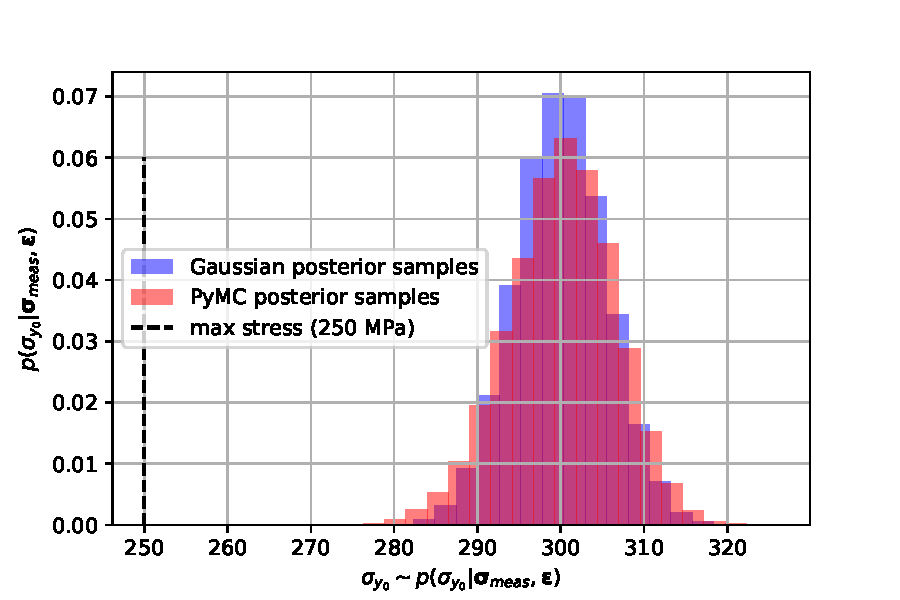
\includegraphics[scale=0.5]{Q3b_3.pdf}
		\caption{Samples from the marginal distribution $ p(\sigma_{y_0} \vert \boldsymbol\sigma_{meas}, \boldsymbol\epsilon)$ over the yield stress.}
		\label{fig:Q3_yield}
	\end{figure}

	The fifth question of interest is: \emph{given the historical data, what is the probability that the measured stress $\sigma_{meas}$ will be more than 200 MPa for a strain of 0.001?} This question can be re-written as: what is the probability $p(\sigma > 200 \vert \epsilon = 0.001, \boldsymbol\sigma_{meas}, \boldsymbol\epsilon)$? This can be expanded through
	\begin{equation}
		\begin{aligned}
		p(\sigma > 200 \vert \epsilon = 0.001, \boldsymbol\sigma_{meas}, \boldsymbol\epsilon) &= 1 - p(\sigma \leq 200 \epsilon = 0.001, \boldsymbol\sigma_{meas}, \boldsymbol\epsilon) \\
		&= 1 - \mathbb{E}_{\sigma_{meas} \sim p(\sigma_{meas} \vert  \epsilon = 0.001, \boldsymbol\sigma_{meas}, \boldsymbol\epsilon)} \{ I(\sigma_{meas} \vert -\infty, 200) \}.
		\end{aligned}
	\end{equation}

	This probability requires samples from the posterior predictive distribution. As such, the sampling procedure to generate posterior predictive samples is as follows:
	\begin{enumerate}
		\item Sample the posterior $\{\boldsymbol{\theta}_i, \eta_i\} \sim p(\boldsymbol{\theta}, \eta \vert \boldsymbol\sigma_{meas}, \boldsymbol\epsilon)$.
		\item Sample the generative model $\sigma_{meas} \sim p(\sigma_{meas} \vert \sigma_l(\boldsymbol\theta_i, \epsilon = 0.001), \eta_i)$.
		\item Repeat
	\end{enumerate} 

	This procedure ensures that we can draw samples from the posterior predictive distribution for $\epsilon = 0.001.$ As initially the noise $\eta$ was unknown, a maximum likelihood estimate of $\eta = 17.149$ for $\boldsymbol\theta = [190 000, 300, 55 000]^T$ MPa. Using the MLE noise, the pre-defined noise ($\eta = 18$), and posterior samples using \texttt{PyMC3}, the probability of interest was found to be
	\begin{enumerate}
		\item $p(\sigma > 200 \vert \epsilon = 0.001, \boldsymbol\sigma_{meas}, \boldsymbol\epsilon)_{pre-defined, \eta = 17.149} = 0.2871$.
		\item $p(\sigma > 200 \vert \epsilon = 0.001, \boldsymbol\sigma_{meas}, \boldsymbol\epsilon)_{pre-defined, \eta = 18} = 0.2956$.
		\item $p(\sigma > 200 \vert \epsilon = 0.001, \boldsymbol\sigma_{meas}, \boldsymbol\epsilon)_{\texttt{PyMC3}} = 0.2835$.
	\end{enumerate}
	Thus, we can conclude that there is a $30\%$ chance that the measured stress will be greater than 200MPa at a strain of 0.001. In Figure \ref{fig:Q3_post_predict_samples}, the three empirical posterior predictive distributions used for this question are shown.
	\begin{figure}[htb!]
		\centering
		\begin{subfigure}[b]{0.3\textwidth}
			\centering
			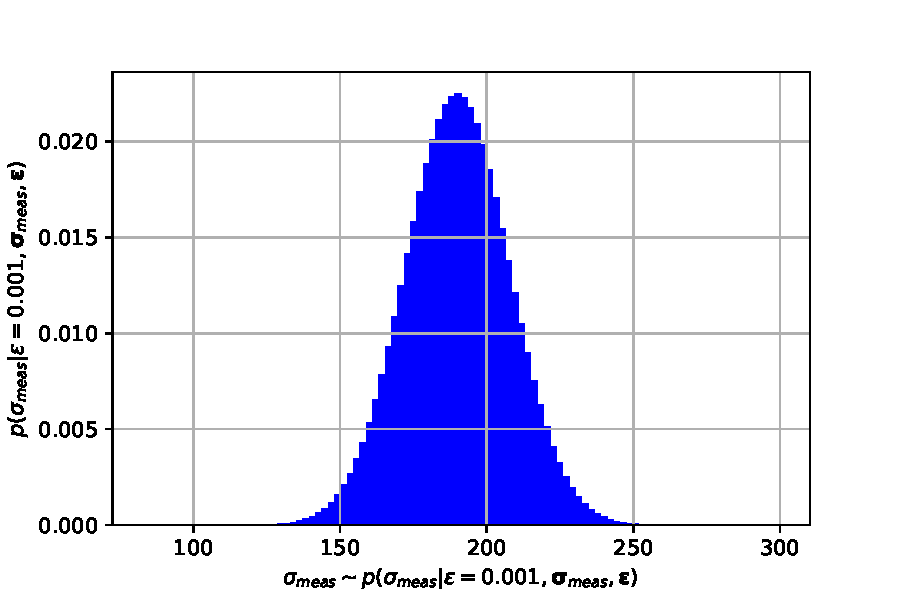
\includegraphics[width=\textwidth]{Q3b_5.pdf}
			\caption{$\eta = 17.149$.}
		\end{subfigure}
		~
		\begin{subfigure}[b]{0.3\textwidth}
			\centering
			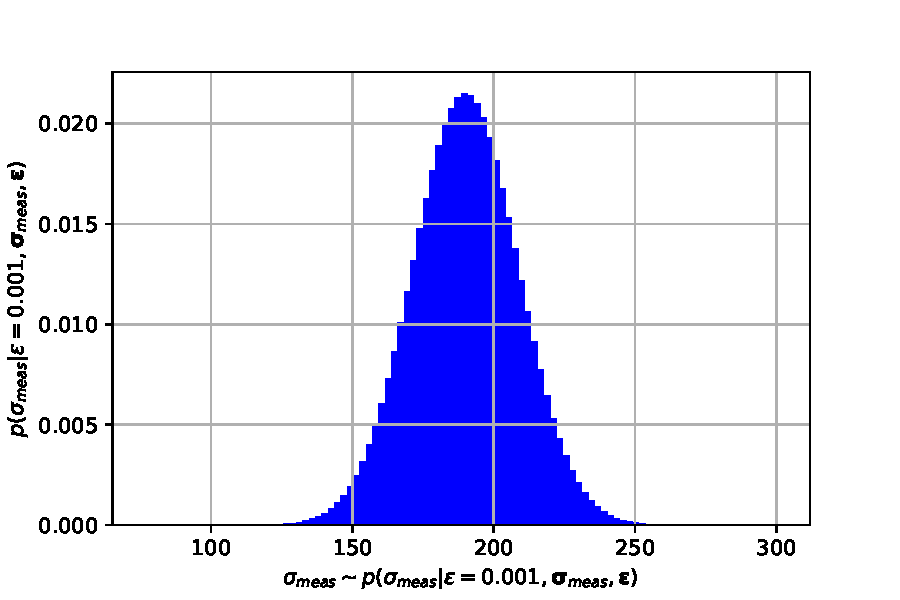
\includegraphics[width=\textwidth]{Q3b_7.pdf}
			\caption{$\eta = 18$.}
		\end{subfigure}
		~
		\begin{subfigure}[b]{0.3\textwidth}
			\centering
			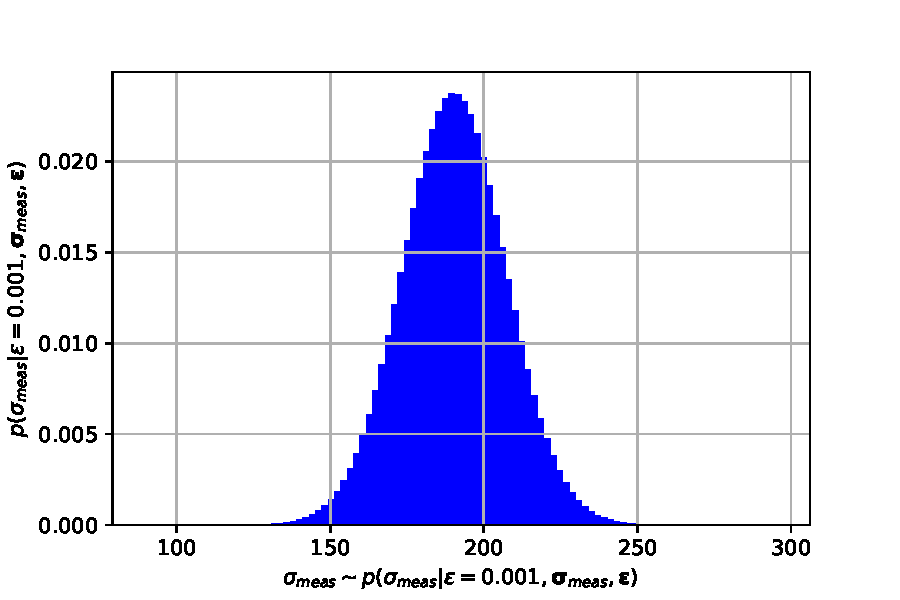
\includegraphics[width=\textwidth]{Q3b_6.pdf}
			\caption{\texttt{PyMC3}.}
		\end{subfigure}
		
		\caption{The empirical posterior predictive distribution where $\epsilon = 0.001$ for three different variations of the posterior predictive distribution.}
		\label{fig:Q3_post_predict_samples}
	\end{figure}


	\clearpage
	
	\section{Question 4}
	
	Dear Dr. Schmidt, 
	
	I have an additional 30 minutes to add in some comments about the fourth question, I figured that I may as well waste my own time and explain my struggles with the fourth question. Before I get into this, I would just like to apologise for needing extra time to finish the assignment, I have no excuses and I am embarrassed that I am in this situation. Please just give me zero for this section and move on with your other work.
	
	My chosen paper was:
	\begin{itemize}
		\item Diamond DH, Heyns PS, Oberholster AJ (2016) Online shaft encoder geometry compensation for arbitrary shaft speed profiles using Bayesian regression. Mech. Syst. Signal Process. 81:402–418
	\end{itemize}
	
	The reason here was simple: I have used the method in this paper in both my Masters and my PhD, and I believe that it is applicable and important to the field. However, in this paper, Dr. Diamond states that the system of equations used is underdetermined and thus a Bayesian approach is used to solve the system. His approach is a based on cubic-spline polynomial regression (to some extent) implementation with a Bayesian regression step to encode some prior information into the problem. I could not understand everything in the paper well enough and quick enough to finish it before today, my apologies for this. 
	
	When I went through the paper I changed one or two of the aspects of his write-up as I could not understand all of his decisions (at least on an intuitive level) and I wanted to check that the system of equations is indeed underdetermined. I attempted to reproduce his derivation and I believe that there is a solution that had a square system of equations and hence should be solvable with a unique solution. I will detail some aspects of this solution some time this evening (graphically and with formal equations), as I cannot figure out if I am wrong (which is the highly probable outcome), or if this is actually something to look into. If you have a second, it would be great if you could tell me where I have or have not made a mistake.
	
	Thanks,
	
	Ryan
	
	\clearpage
	
	
	
	\iffalse
	%General figure information
	\begin{figure}[htb!]
		\centering
		\includegraphics[scale=0.5]{.pdf}
		\caption{words words words.}
		\label{fig:}
	\end{figure}
	
	\begin{figure}[htb!]
		\centering
		\begin{subfigure}[b]{0.45\textwidth}
			\centering
			\includegraphics[width=\textwidth]{.pdf}
			\caption{sub-words.}
		\end{subfigure}
		~
		\begin{subfigure}[b]{0.45\textwidth}
			\centering
			\includegraphics[width=\textwidth]{.pdf}
			\caption{sub-words.}
		\end{subfigure}
		
		\caption{words words words.}
		\label{fig:}
	\end{figure}
	
	\fi
	
	\clearpage
	
	%Print the bibliography
	\printbibliography
	
\end{document}